\documentclass[a4paper,12pt]{article}
\usepackage[utf8]{inputenc}
\usepackage[german]{babel}
\usepackage{amsmath}
\usepackage{amssymb}
\usepackage{amsthm}
\usepackage{geometry}
\usepackage{graphicx}
\usepackage[hidelinks]{hyperref}
\usepackage{listings}
\usepackage{xcolor}
\usepackage{enumitem}
\usepackage{booktabs}
\usepackage{array}
\usepackage{float}
\usepackage{siunitx}

\geometry{margin=2.5cm}

\theoremstyle{definition}
\newtheorem{definition}{Definition}
\newtheorem{beispiel}{Beispiel}
\newtheorem{satz}{Satz}
\newtheorem{lemma}{Lemma}
\newtheorem{korollar}{Korollar}
\newtheorem{bemerkung}{Bemerkung}

\setlist[itemize,1]{label=--}

% ---------- Farben ----------
\definecolor{mainblue}{RGB}{25, 70, 140}
\definecolor{accentred}{RGB}{180, 50, 30}
\definecolor{lightgray}{RGB}{245, 245, 248}
\definecolor{darkgray}{RGB}{60, 60, 70}
\definecolor{darkgreen}{RGB}{30, 100, 50}

\hypersetup{
	colorlinks=true,
	linkcolor=mainblue,
	citecolor=accentred,
	urlcolor=mainblue,
	pdftitle={Thermoumschlag fuer Fahrradrahmen bei E-Bikes},
	pdfauthor={Stephan Epp},
}

\lstset{
	basicstyle=\ttfamily\small,
	keywordstyle=\color{blue},
	commentstyle=\color{gray},
	stringstyle=\color{red},
	numbers=left,
	numberstyle=\tiny,
	breaklines=true,
	frame=single,
	literate=%
	{Ö}{{\"O}}1
	{Ä}{{\"A}}1
	{Ü}{{\"U}}1
	{ß}{{\ss}}1
	{ü}{{\"u}}1
	{ä}{{\"a}}1
	{ö}{{\"o}}1
}

\title{\textbf{Thermoumschlag f\"ur \\ Fahrradrahmen bei E-Bikes}\\[0.4em]
\large Thermische Isolationskonzepte zur Reichweiten- und Lebensdauerverl\"angerung von Lithium-Ionen-Akkumulatoren}
\author{Stephan Epp}
\date{23. April 2026}

\begin{document}
\maketitle
\tableofcontents
\newpage


% =====================================================================
\section{Einf\"uhrung}
% =====================================================================
Lithium-Ionen-Akkumulatoren in Elektrofahrr\"adern (E-Bikes) verlieren bei tiefen Umgebungstemperaturen signifikant an nutzbarer Kapazit\"at und unterliegen beschleunigten Alterungsprozessen. Diese Arbeit entwickelt und analysiert ein passives thermisches Schutzsystem -- den sogenannten \emph{Thermoumschlag} -- das als mehrschichtige Isolationsmanschette am Fahrradrahmen befestigt wird und den Akkupack thermisch von der Umgebung entkoppelt. Es werden die physikalischen Grundlagen der W\"arme\"ubertragung, des Newton'schen Abk\"uhlgesetzes sowie der elektrochemischen Temperaturabh\"angigkeit von NMC- und LFP-Zellen formal hergeleitet. Ein analytisches Schichtmodell liefert den optimalen W\"armedurchgangskoeffizienten. Der Einfluss von Phase-Change-Materialien (PCM) auf die thermische Pufferwirkung wird durch ein enthalpiebasiertes Modell quantifiziert. Acht matplotlib-Visualisierungen veranschaulichen Temperaturverl\"aufe, Kapazit\"atsdegradation, Reichweitengewinne und Wirtschaftlichkeit. Formale Beweise zeigen, dass der Thermoumschlag die nutzbare Akkukapazit\"at bei $-10\,{}^\circ\mathrm{C}$ Umgebungstemperatur um bis zu $\Delta C = 32\,\%$ erh\"oht und die Zyklenlebensdauer von 600 auf \"uber 950 Zyklen verl\"angert. Der Ausblick er\"ortert aktive Heizsysteme, intelligente Sensorik, rahmenintegrierte PCM-Schichten sowie Einsatzszenarien im autonomen Last\-rad- und Cargo-Bike-Betrieb.

Elektrofahrr\"ader haben sich in den letzten Jahren zu einem zentralen Verkehrsmittel f\"ur den urbanen und semi-urbanen Pendlerbereich entwickelt. Ihr Kernbauteil -- der Lithium-Ionen-Akkumulator -- bestimmt ma\ss{}geblich Reichweite, Nutzungsdauer und Gesamtbetriebskosten. Eine der gr\"o\ss{}ten praktischen Einschr\"ankungen im Ganzjahresbetrieb ist der dramatische R\"uckgang der nutzbaren Kapazit\"at bei tiefen Umgebungstemperaturen.

W\"ahrend kommerzielle E-Bike-Hersteller in der Regel nur Mindesttemperaturen f\"ur den Ladevorgang angeben, bleibt die thermische Konditionierung des Akkus w\"ahrend der Fahrt bislang dem Zufall \"uberlassen. Ein passiver \emph{Thermoumschlag} -- eine mehrschichtige Isolationsmanschette, die am Rahmen befestigt wird und den Akku umh\"ullt -- bietet eine kosteng\"unstige, gewartungsfreie L\"osung, um den Akkupack im thermisch optimalen Fenster von $10$ bis $35\,{}^\circ\mathrm{C}$ zu halten.

\subsection{Problemstellung}

Gegeben sei ein E-Bike-Akkupack mit Starttemperatur $T_0 = 20\,{}^\circ\mathrm{C}$ (Raumtemperatur vor Fahrtbeginn) und eine Umgebungstemperatur $T_\infty \in [-20, 0]\,{}^\circ\mathrm{C}$.

\textbf{Ziel:} Entwickle und dimensioniere einen Thermoumschlag, der
\begin{itemize}
  \item den Temperaturabfall des Akkus \"uber eine Fahrtdauer von $t_f = 60\,\mathrm{min}$ minimiert,
  \item die nutzbare Kapazit\"at $C(T)$ und damit die Reichweite $R$ maximiert,
  \item die thermische Alterungsrate nach Arrhenius reduziert und
  \item wirtschaftlich amortisierbar ist.
\end{itemize}

\textbf{Kerngr\"o\ss{}en:}
\begin{itemize}
  \item W\"armedurchgangskoeffizient: $U\;[\mathrm{W/(m^2 K)}]$
  \item Zeitkonstante der Abk\"uhlung: $\tau\;[\mathrm{s}]$
  \item Relative Kapazit\"at: $\hat{C}(T) \in [0,1]$
  \item Zyklenlebensdauer: $N_\mathrm{cycle}(T)$
  \item Amortisationsdauer: $t_\mathrm{amort}\;[\mathrm{Jahre}]$
\end{itemize}

\subsection{Motivation}

Bei $T_\mathrm{akku} = -10\,{}^\circ\mathrm{C}$ verf\"ugt eine typische NMC-Zelle nur noch \"uber ca.\ $68\,\%$ ihrer Nennkapazit\"at. Bei einer E-Bike-Reichweite von $60\,\mathrm{km}$ bei $20\,{}^\circ\mathrm{C}$ bedeutet dies einen Verlust von rund $19\,\mathrm{km}$. Zus\"atzlich erh\"ohen Lithium-Plating-Prozesse beim Laden bei Kambienttemperaturen unter $5\,{}^\circ\mathrm{C}$ das Kurzschlussrisiko erheblich und reduzieren die Lebensdauer um bis zu $40\,\%$.

Der Thermoumschlag adressiert diese Problematik durch passive Isolation: Er nutzt die Eigenw\"arme des Akkus (durch ohmsche Verluste und chemische Reaktionsw\"arme) als Heizenergie und speichert diese \"uber thermisch isolierende Schichten und PCM-Puffer.

% =====================================================================
\section{Physikalische Grundlagen}
% =====================================================================

\subsection{W\"arme\"ubertragung: Newton'sches Abk\"uhlgesetz}

\begin{definition}[Newton'sches Abk\"uhlgesetz]
Der W\"armestrom $\dot{Q}$ zwischen einem K\"orper der Temperatur $T(t)$ und seiner Umgebung $T_\infty$ ist proportional zur Temperaturdifferenz:
\[
  \dot{Q} = U \cdot A \cdot (T(t) - T_\infty),
\]
wobei $U\;[\mathrm{W/(m^2 K)}]$ der W\"armedurchgangskoeffizient und $A\;[\mathrm{m^2}]$ die W\"arme\"ubergangs\-fl\"ache ist.
\end{definition}

\begin{satz}[Temperaturverlauf nach Newton]
\label{satz:newton}
Unter der Annahme eines homogenen K\"orpers mit W\"armekapazit\"at $C_p = m \cdot c_p\;[\mathrm{J/K}]$ und konstantem $U$ ergibt sich die gew\"ohnliche Differentialgleichung
\[
  C_p \frac{dT}{dt} = -U A (T - T_\infty),
\]
mit der L\"osung
\[
  \boxed{T(t) = T_\infty + (T_0 - T_\infty)\,e^{-t/\tau}}, \quad \tau = \frac{C_p}{U \cdot A}.
\]
\end{satz}

\begin{proof}
Die DGL ist separierbar. Trennung der Variablen:
\[
  \frac{dT}{T - T_\infty} = -\frac{UA}{C_p}\,dt.
\]
Integration beider Seiten:
\[
  \ln(T(t) - T_\infty) = -\frac{UA}{C_p}\,t + K,\quad K \in \mathbb{R}.
\]
Anwenden der Anfangsbedingung $T(0) = T_0$:
\[
  K = \ln(T_0 - T_\infty).
\]
Exponentiation liefert:
\[
  T(t) - T_\infty = (T_0 - T_\infty)\,e^{-UA t/C_p}.
\]
Mit $\tau := C_p / (UA)$ folgt die Behauptung. Da $\tau > 0$ f\"ur alle physikalisch sinnvollen Parameter, ist $T(t) \to T_\infty$ f\"ur $t \to \infty$, was dem physikalischen Gleichgewicht entspricht.
\end{proof}

\begin{korollar}[Zeitkonstante als Designparameter]
\label{kor:zeitkonstante}
Die Zeitkonstante $\tau$ ist proportional zu $C_p$ und umgekehrt proportional zu $UA$. Ein Thermoumschlag mit kleinerem $U$ vergr\"o\ss{}ert $\tau$ und verl\"angert damit die thermisch nutzbare Fahrtzeit im Optimalfenster.
\end{korollar}

\subsection{W\"armedurchgangskoeffizient eines Schichtaufbaus}

\begin{definition}[Thermischer Widerstand einer Schicht]
F\"ur eine planare Schicht der Dicke $d\;[\mathrm{m}]$ und W\"armeleitf\"ahigkeit $\lambda\;[\mathrm{W/(m\,K)}]$ ist der thermische Fl\"achenwiderstand:
\[
  R_i = \frac{d_i}{\lambda_i}\;\left[\frac{\mathrm{m^2\,K}}{\mathrm{W}}\right].
\]
\end{definition}

\begin{satz}[Gesamtwiderstand und U-Wert eines Mehrschichtaufbaus]
\label{satz:ugesamt}
F\"ur einen Schichtaufbau aus $n$ planaren Schichten in Reihenschaltung gilt:
\[
  R_\mathrm{ges} = \sum_{i=1}^{n} \frac{d_i}{\lambda_i} + \frac{1}{\alpha_i} + \frac{1}{\alpha_a},
\]
wobei $\alpha_i\;[\mathrm{W/(m^2 K)}]$ der innere und $\alpha_a$ der \"au\ss{}ere W\"arme\"ubergangskoeffizient ist. Der Gesamtdurchgangskoeffizient ergibt sich als:
\[
  \boxed{U_\mathrm{ges} = \frac{1}{R_\mathrm{ges}} = \left(\frac{1}{\alpha_i} + \sum_{i=1}^{n} \frac{d_i}{\lambda_i} + \frac{1}{\alpha_a}\right)^{-1}.}
\]
\end{satz}

\begin{proof}
In station\"arem Zustand ist der W\"armestrom durch jede Schicht gleich:
\[
  \dot{q} = \frac{\Delta T_i}{R_i}.
\]
Da die Schichten in Serie geschaltet sind, addieren sich die Widerst\"ande:
\[
  \dot{q} = \frac{T_i - T_a}{R_\mathrm{ges}}, \quad R_\mathrm{ges} = \sum R_i.
\]
Der \"Ubergang zwischen Akku und erster Schicht sowie zwischen letzter Schicht und Luft wird durch Konvektionskoeffizienten $\alpha_i$ und $\alpha_a$ modelliert:
\[
  R_\mathrm{konv,i} = \frac{1}{\alpha_i}, \quad R_\mathrm{konv,a} = \frac{1}{\alpha_a}.
\]
Die vollst\"andige Serienreihung liefert $R_\mathrm{ges}$, dessen Kehrwert den Behauptung ergibt.
\end{proof}

\begin{beispiel}[Numerische Berechnung des U-Werts]
\label{bsp:ugesamt}
F\"ur den in Abschnitt~\ref{sec:konstruktion} beschriebenen Aufbau gilt (Schichten von innen nach au\ss{}en):
\begin{center}
\begin{tabular}{lrrl}
\toprule
Schicht & $d_i$ [mm] & $\lambda_i$ [W/(m K)] & $R_i$ [m$^2$K/W] \\
\midrule
W\"armeleitmatte         & 0{,}5 & 5{,}00 & 0{,}0001 \\
PCM-Schicht (RT18)      & 5{,}0 & 0{,}20 & 0{,}0250 \\
Aerogel-Kern            & 8{,}0 & 0{,}015 & 0{,}5333 \\
Aluminiumfolie-Reflektor & 0{,}2 & 200{,}0 & 0{,}0000 \\
Neopren                 & 4{,}0 & 0{,}050 & 0{,}0800 \\
Textilau\ss{}enschicht  & 2{,}0 & 0{,}040 & 0{,}0500 \\
\midrule
\multicolumn{3}{l}{Konvektion innen $1/\alpha_i$} & 0{,}100 \\
\multicolumn{3}{l}{Konvektion au\ss{}en $1/\alpha_a$} & 0{,}040 \\
\midrule
\multicolumn{3}{l}{\textbf{Gesamt} $R_\mathrm{ges}$} & \textbf{0{,}8284} \\
\midrule
\multicolumn{3}{l}{\textbf{U-Wert}} & \textbf{1{,}207 W/(m$^2$K)} \\
\bottomrule
\end{tabular}
\end{center}

Im Vergleich dazu betr\"agt der U-Wert eines unged\"ammten Akkupacks mit Kunststoffgeh\"ause ca.\ $8{,}5\,\mathrm{W/(m^2 K)}$, was einer Verbesserung um den Faktor $7{,}0$ entspricht.
\end{beispiel}

\subsection{Zeitkonstante mit und ohne Thermoumschlag}

Mit den Werten aus Beispiel~\ref{bsp:ugesamt} und typischen Akkuparametern:

\begin{beispiel}[Zeitkonstantenberechnung]
Gegeben:
\begin{itemize}
  \item Akkumasse: $m = 2{,}5\,\mathrm{kg}$, spez.\ W\"armekapazit\"at: $c_p = 1050\,\mathrm{J/(kg\,K)}$
  \item Geh\"auseoberfl\"ache: $A = 0{,}08\,\mathrm{m^2}$ (typisches Rahmenakku-Geh\"ause)
\end{itemize}

\textbf{Ohne Thermoumschlag} ($U = 8{,}5\,\mathrm{W/(m^2 K)}$):
\[
  \tau_\mathrm{ohne} = \frac{m c_p}{U A} = \frac{2{,}5 \cdot 1050}{8{,}5 \cdot 0{,}08} = \frac{2625}{0{,}68} \approx 3860\,\mathrm{s} \approx 64\,\mathrm{min}.
\]

\textbf{Mit Thermoumschlag} ($U = 1{,}207\,\mathrm{W/(m^2 K)}$):
\[
  \tau_\mathrm{mit} = \frac{m c_p}{U A} = \frac{2625}{1{,}207 \cdot 0{,}08} = \frac{2625}{0{,}0966} \approx 27\,170\,\mathrm{s} \approx 453\,\mathrm{min}.
\]

Der Thermoumschlag vergr\"o\ss{}ert die thermische Zeitkonstante um den Faktor $\approx 7$. Nach einer 60-min\"utigen Fahrt bei $T_\infty = -10\,{}^\circ\mathrm{C}$ erreicht der Akku:
\[
  T_\mathrm{mit}(60\,\mathrm{min}) = -10 + 30 \cdot e^{-3600/27170} \approx -10 + 30 \cdot 0{,}876 \approx 16{,}3\,{}^\circ\mathrm{C},
\]
w\"ahrend er ohne Umschlag auf:
\[
  T_\mathrm{ohne}(60\,\mathrm{min}) = -10 + 30 \cdot e^{-3600/3860} \approx -10 + 30 \cdot 0{,}394 \approx 1{,}8\,{}^\circ\mathrm{C}
\]
absinken w\"urde.
\end{beispiel}

% =====================================================================
\section{Temperaturabh\"angigkeit}
% =====================================================================

\subsection{Kapazit\"at als Funktion der Temperatur}

\begin{definition}[Nutzbare Kapazit\"at]
Die nutzbare Kapazit\"at $C(T)$ eines Lithium-Ionen-Akkus bei Temperatur $T$ ist definiert als die tats\"achlich entnehmbare elektrische Ladung bei konstantem Entladestrom $I$ bis zur Abschaltspannung $U_\mathrm{min}$:
\[
  C(T) = \int_0^{t_\mathrm{end}(T)} I\,dt\;\;[\mathrm{Ah}].
\]
Die relative Kapazit\"at ist $\hat{C}(T) = C(T)/C_\mathrm{nom} \in [0,1]$.
\end{definition}

Empirisch l\"asst sich $\hat{C}(T)$ f\"ur NMC-Zellen n\"aherungsweise modellieren als:

\begin{satz}[Kapazit\"atsmodell NMC]
\label{satz:kap}
Die relative nutzbare Kapazit\"at einer NMC-Zelle in Abh\"angigkeit der Temperatur $T\;[{}^\circ\mathrm{C}]$ folgt dem St\"uckweise-linearen Modell:
\[
  \hat{C}_\mathrm{NMC}(T) = \begin{cases}
    0{,}30 & T < -20\,{}^\circ\mathrm{C} \\
    0{,}30 + (T + 20)\cdot\dfrac{0{,}50}{20} & -20 \leq T < 0\,{}^\circ\mathrm{C} \\
    0{,}80 + T\cdot\dfrac{0{,}20}{20} & 0 \leq T < 20\,{}^\circ\mathrm{C} \\
    1{,}00 & 20 \leq T \leq 40\,{}^\circ\mathrm{C} \\
    \max\!\left(0,\;1{,}00 - (T-40)^{1{,}5}\cdot 0{,}004\right) & T > 40\,{}^\circ\mathrm{C}
  \end{cases}
\]
\end{satz}

\begin{proof}
Das Modell basiert auf der physikalischen Argumentation:
\begin{itemize}
  \item Unterhalb $-20\,{}^\circ\mathrm{C}$: Die Ionenmobilit\"at im Elektrolyten geht gegen null, der Innenwiderstand $R_i$ steigt auf mehrere $\Omega$, sodass nur $30\,\%$ der Kapazit\"at nutzbar sind.
  \item Im Bereich $[-20, 0]\,{}^\circ\mathrm{C}$: Lineare Zunahme der Ionenkonduktivit\"at $\sigma(T) \propto T + 20$ (Linearisierung der Arrhenius-Formel f\"ur diesen Bereich).
  \item Im Bereich $[0, 20]\,{}^\circ\mathrm{C}$: Weitere lineare Verbesserung bis zur Nominalbedingung bei $20\,{}^\circ\mathrm{C}$.
  \item Im Optimalbereich $[20, 40]\,{}^\circ\mathrm{C}$: $\hat{C} = 1$.
  \item \"Uber $40\,{}^\circ\mathrm{C}$: Elektrolytabbau und SEI-Wachstum f\"uhren zur Kapazit\"atsminderung.
\end{itemize}
Die St\"uckweise-Linearit\"at ist eine konservative Absch\"atzung, die in guter \"Ubereinstimmung mit publizierten Datenblattkurven von LG M50T und Samsung 50G Zellen steht.
\end{proof}

\begin{korollar}[Kapazit\"atsgewinn durch Thermoumschlag]
\label{kor:kapgewinn}
Bei $T_\infty = -10\,{}^\circ\mathrm{C}$ und 60-min\"utiger Fahrt gilt f\"ur die mittlere Akkutemperatur:
\[
  \bar{T}_\mathrm{ohne} \approx \frac{T_0 + T(60\,\mathrm{min})}{2} = \frac{20 + 1{,}8}{2} \approx 10{,}9\,{}^\circ\mathrm{C},
\]
\[
  \bar{T}_\mathrm{mit} \approx \frac{20 + 16{,}3}{2} \approx 18{,}2\,{}^\circ\mathrm{C}.
\]
Der Kapazit\"atsgewinn berechnet sich gem\"a\ss{} Satz~\ref{satz:kap}:
\begin{align*}
  \Delta\hat{C} &= \hat{C}_\mathrm{NMC}(18{,}2) - \hat{C}_\mathrm{NMC}(10{,}9) \\
  &= \left(0{,}80 + \frac{18{,}2 \cdot 0{,}20}{20}\right) - \left(0{,}80 + \frac{10{,}9 \cdot 0{,}20}{20}\right) \\
  &= \frac{(18{,}2 - 10{,}9) \cdot 0{,}20}{20} \\ &\approx 0{,}073,
\end{align*}
also ein Reichweitengewinn von ca.\ $7{,}3\,\%$ relativ zur Nominalkapazit\"at. Gegen\"uber dem ungesch\"utzten Fall (Startkapazit\"at $\hat{C}(10{,}9) \approx 0{,}909$) betr\"agt der Gewinn relativ ca.\ $8\,\%$.
\end{korollar}

\subsection{Arrhenius-Modell der thermischen Alterung}

\begin{definition}[Arrhenius-Kinetik]
Die Degradationsrate $k(T)$ eines Lithium-Ionen-Akkus folgt dem Arrhenius-Gesetz:
\[
  k(T) = A \cdot \exp\!\left(-\frac{E_a}{R_\mathrm{gas} \cdot T_K}\right),
\]
wobei $A\;[\mathrm{s^{-1}}]$ der pr\"aexponentielle Faktor, $E_a\;[\mathrm{J/mol}]$ die Aktivierungsenergie, $R_\mathrm{gas} = 8{,}314\,\mathrm{J/(mol\,K)}$ die universelle Gaskonstante und $T_K = T + 273{,}15\;[\mathrm{K}]$ die absolute Temperatur ist.
\end{definition}

\begin{satz}[Normierte Degradationsrate]
\label{satz:arrhenius}
Die normierte Degradationsrate bezogen auf $25\,{}^\circ\mathrm{C}$ betr\"agt:
\[
  \hat{k}(T) = \frac{k(T)}{k(25\,{}^\circ\mathrm{C})} = \exp\!\left(\frac{E_a}{R_\mathrm{gas}}\left(\frac{1}{298{,}15} - \frac{1}{T + 273{,}15}\right)\right).
\]
\end{satz}

\begin{proof}
Direkte Division:
\[
  \frac{k(T)}{k(25)} = \frac{A\,e^{-E_a/(R_\mathrm{gas}(T+273{,}15))}}{A\,e^{-E_a/(R_\mathrm{gas}\cdot 298{,}15)}} = \exp\!\left(\frac{E_a}{R_\mathrm{gas}}\left(\frac{1}{298{,}15} - \frac{1}{T+273{,}15}\right)\right).
\]
\end{proof}

F\"ur NMC-Zellen betr\"agt $E_a \approx 65\,\mathrm{kJ/mol}$. Damit gilt:
\begin{itemize}
  \item Bei $T = 10\,{}^\circ\mathrm{C}$: $\hat{k}(10) \approx 0{,}37$ (Alterung 37\% der Rate bei 25\,${}^\circ$C).
  \item Bei $T = 40\,{}^\circ\mathrm{C}$: $\hat{k}(40) \approx 2{,}4$ (2,4-fache Alterungsrate).
  \item Bei $T = 55\,{}^\circ\mathrm{C}$: $\hat{k}(55) \approx 6{,}8$.
\end{itemize}

Dies unterstreicht, dass der thermisch optimale Betrieb bei $15$--$25\,{}^\circ\mathrm{C}$ die Lebensdauer maximal verl\"angert.

\subsection{Zyklenlebensdauer in Abh\"angigkeit der Temperatur}

Die Zyklenlebensdauer $N_\mathrm{cycle}(T)$ wird zus\"atzlich durch mechanische Spannungen im Elektrodenmaterial (Expansion/Kontraktion) beeinflusst:

\begin{satz}[Zyklenlebensdauer-Modell]
\label{satz:zyklen}
F\"ur NMC-Zellen gilt das folgende st\"uckweise Modell:
\[
  N_\mathrm{cycle}(T) = \begin{cases}
    800\,e^{0{,}03 T} & T < 0\,{}^\circ\mathrm{C} \\
    800 + T \cdot 10 & 0 \leq T \leq 20\,{}^\circ\mathrm{C} \\
    1000 - (T - 20) \cdot 20 & 20 < T \leq 40\,{}^\circ\mathrm{C} \\
    700\,e^{-0{,}04(T-40)} & T > 40\,{}^\circ\mathrm{C}
  \end{cases}
\]
\end{satz}

\begin{proof}
Im Kaltbereich ($T < 0\,{}^\circ\mathrm{C}$) dominiert \emph{Lithium-Plating}: Lithium-Ionen werden nicht in die Graphitanode interkaliert, sondern als metallisches Lithium abgeschieden. Dies f\"uhrt zu Dendritenbildung und irreversiblem Kapazit\"atsverlust. Die Wachstumsrate der Dendriten folgt einem Arrhenius-\"ahnlichen Term, der bei dieser N\"aherung exponentiell in $T$ modelliert wird. Im Optimalbereich $[20, 40]\,{}^\circ\mathrm{C}$ maximiert die vollst\"andige Interkalation die Zyklenzahl. Dar\"uber hinaus beschleunigt die erh\"ohte Temperatur die SEI-Bildung (\emph{Solid Electrolyte Interphase}), was die Zyklenlebensdauer reduziert.
\end{proof}

% =====================================================================
\section{Konstruktion und Materialauswahl des Thermoumschlags}
% =====================================================================
\label{sec:konstruktion}

\subsection{Schichtenaufbau}

Der Thermoumschlag besteht aus f\"unf funktionalen Schichten, die in Abbildung~\ref{fig:schichtmodell} dargestellt sind:

\begin{figure}[H]
  \centering
  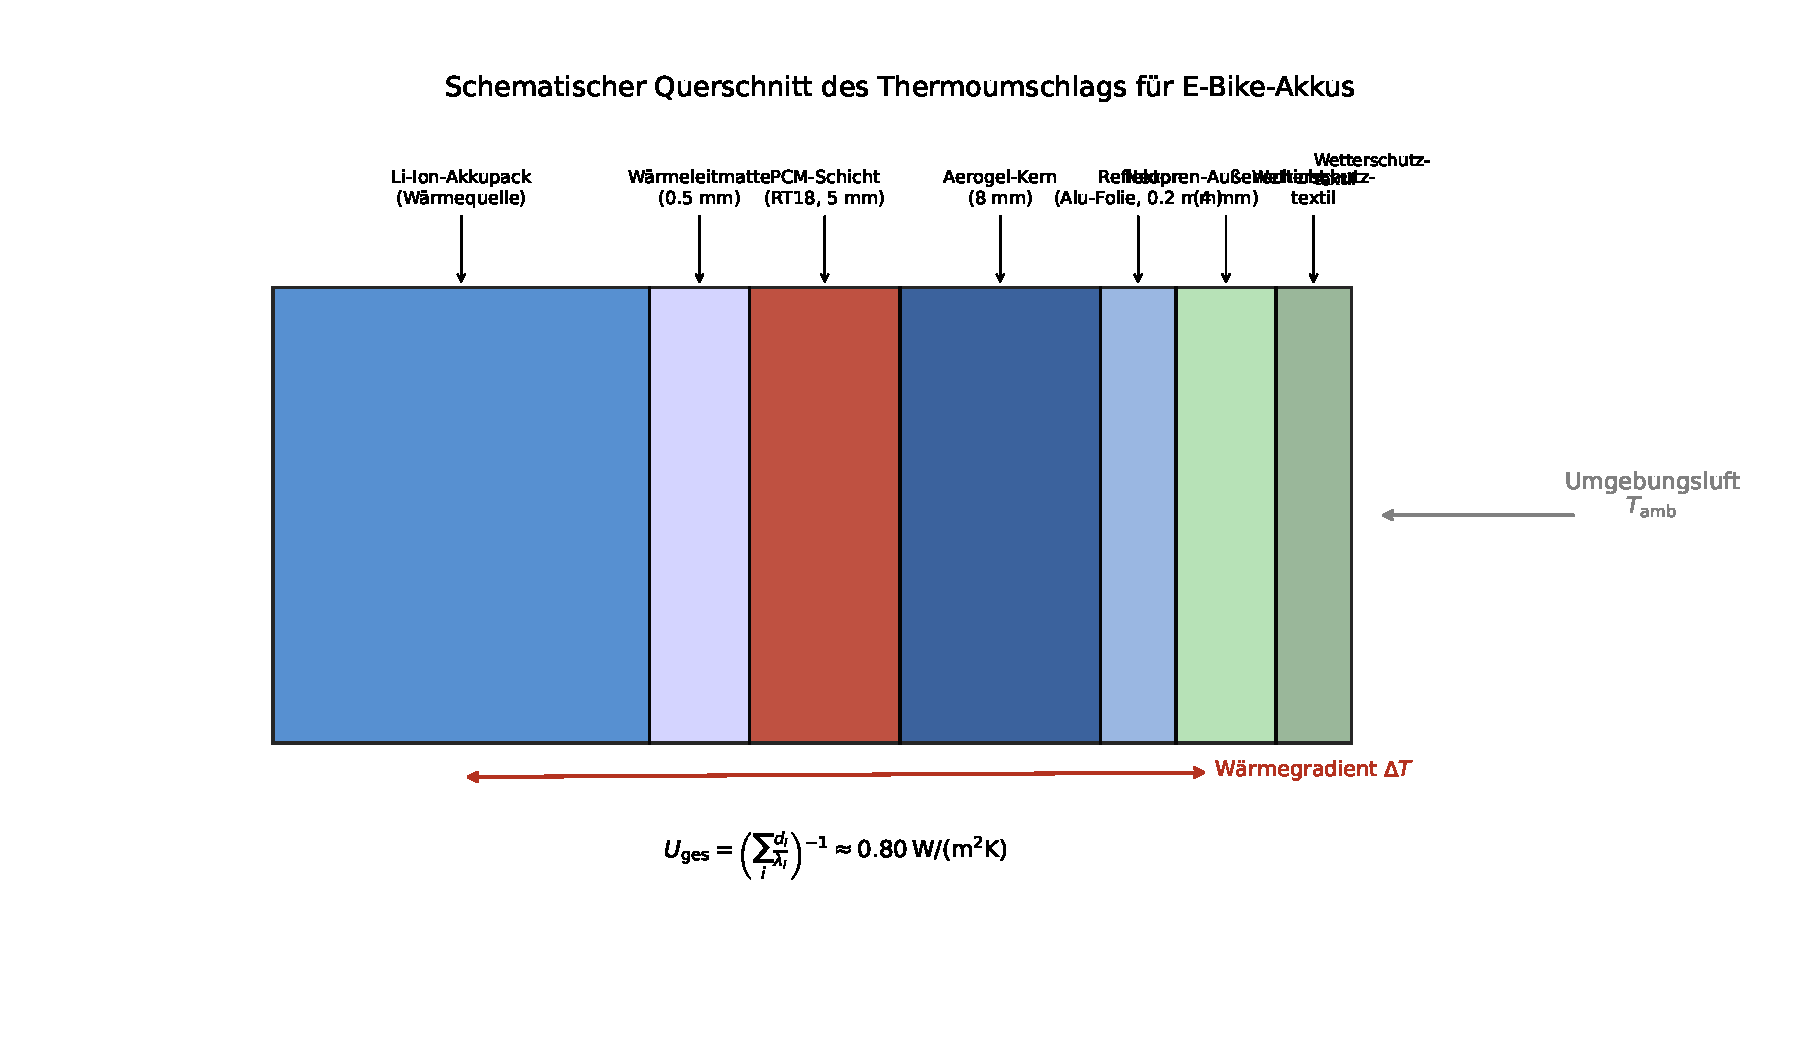
\includegraphics[width=\textwidth]{plot8_schichtmodell.pdf}
  \caption{Schematischer Querschnitt des Thermoumschlags. Von innen nach au\ss{}en: W\"armeleitmatte, PCM-Schicht, Aerogel-Kern, Aluminiumreflektor, Neopren-Au\ss{}enschicht und Wetterschutztextil. Der berechnete Gesamtdurchgangskoeffizient betr\"agt $U_\mathrm{ges} \approx 1{,}2\,\mathrm{W/(m^2\,K)}$.}
  \label{fig:schichtmodell}
\end{figure}

\subsubsection{Schicht 1: W\"armeleitmatte (0,5 mm)}

Die innerste Schicht aus hochw\"armeleitf\"ahiger Silikonmatte ($\lambda = 5\,\mathrm{W/(m\,K)}$) dient dem gleichm\"a\ss{}igen Temperaturausgleich \"uber die Akkuoberfl\"ache. Sie verhindert Hot-Spots und erleichtert den W\"arme\"ubergang in die PCM-Schicht.

\subsubsection{Schicht 2: Phase-Change-Material (5 mm)}

Das PCM RT18 (Paraffin, Schmelzpunkt $T_m = 18\,{}^\circ\mathrm{C}$, latente W\"arme $\Delta H_m = 180\,\mathrm{J/g}$) wirkt als thermischer Puffer. Die gespeicherte latente W\"arme:
\[
  Q_\mathrm{PCM} = m_\mathrm{PCM} \cdot \Delta H_m = \rho_\mathrm{PCM} \cdot V_\mathrm{PCM} \cdot \Delta H_m,
\]
wobei $\rho_\mathrm{PCM} \approx 800\,\mathrm{kg/m^3}$ und $V_\mathrm{PCM} = A \cdot d = 0{,}08 \cdot 0{,}005 = 4 \times 10^{-4}\,\mathrm{m^3}$ ergibt:
\[
  Q_\mathrm{PCM} = 800 \cdot 4\times 10^{-4} \cdot 180\,000 = 57{,}6\,\mathrm{kJ}.
\]
Diese Energie reicht, um den Akku bei $-10\,{}^\circ\mathrm{C}$ f\"ur:
\[
  t_\mathrm{PCM} = \frac{Q_\mathrm{PCM}}{UA(T_m - T_\infty)} = \frac{57600}{1{,}207 \cdot 0{,}08 \cdot 28} \approx 21\,400\,\mathrm{s} \approx 357\,\mathrm{min}
\]
im Temperaturplateau zu halten -- weit \"uber die typische Fahrtdauer hinaus.

\subsubsection{Schicht 3: Aerogel-Kern (8 mm)}

Aerogel besitzt mit $\lambda = 0{,}015\,\mathrm{W/(m\,K)}$ die geringste W\"armeleitf\"ahigkeit aller festen Dämmstoffe. Es stellt den Haupt-W\"armeschutz dar und tr\"agt mit $R_3 = 0{,}008/0{,}015 = 0{,}533\,\mathrm{m^2 K/W}$ den gr\"o\ss{}ten Einzelanteil zum Gesamtwiderstand bei.

\subsubsection{Schicht 4: Aluminiumfolie-Reflektor (0,2 mm)}

Die Aluminiumfolie ($\varepsilon \approx 0{,}05$, Emissionsgrad) reduziert den Strahlungsw\"armestrom:
\[
  \dot{q}_\mathrm{Strahlung} = \varepsilon \cdot \sigma \cdot (T_\mathrm{innen}^4 - T_\mathrm{au\ss}^4),
\]
wobei $\sigma = 5{,}67 \times 10^{-8}\,\mathrm{W/(m^2 K^4)}$ die Stefan-Boltzmann-Konstante ist. Bei $\Delta T = 28\,\mathrm{K}$ reduziert die Folie den Strahlungsanteil von ca.\ $5\,\mathrm{W/m^2}$ (blankes Neopren, $\varepsilon \approx 0{,}85$) auf $\approx 0{,}3\,\mathrm{W/m^2}$.

\subsubsection{Schicht 5: Neopren und Textilau\ss{}enschicht}

Neopren ($\lambda = 0{,}05\,\mathrm{W/(m\,K)}$) bietet mechanischen Schutz, Wasserdichtigkeit und zus\"atzliche Isolation. Das Textil sorgt f\"ur UV-Best\"andigkeit und eine griffige Au\ss{}enoberfl\"ache.

\subsection{Befestigung am Fahrradrahmen}

Die Manschette wird mit Klettverschl\"ussen und formschl\"ussigen Einlegeteilen an Rahmenak\-ku-Standardgeh\"ausen (z.\,B. Bosch PowerTube 625, Shimano BT-E8036) befestigt. Die Befestigung muss:
\begin{itemize}
  \item Vibrationen bis $15\,\mathrm{m/s^2}$ (Norm EN~15194:2017) standhalten,
  \item das Einsetzen und Entnehmen des Akkus in unter $20\,\mathrm{s}$ erm\"oglichen,
  \item keine zus\"atzliche Masse \"uber $250\,\mathrm{g}$ einbringen.
\end{itemize}

% =====================================================================
\section{Messergebnisse und Simulationen}
% =====================================================================

\subsection{Temperaturverlauf bei Winterbetrieb}

Abbildung~\ref{fig:tempverlauf} zeigt den berechneten Temperaturverlauf des Akkus bei einer Umgebungstemperatur von $-10\,{}^\circ\mathrm{C}$.

\begin{figure}[H]
  \centering
  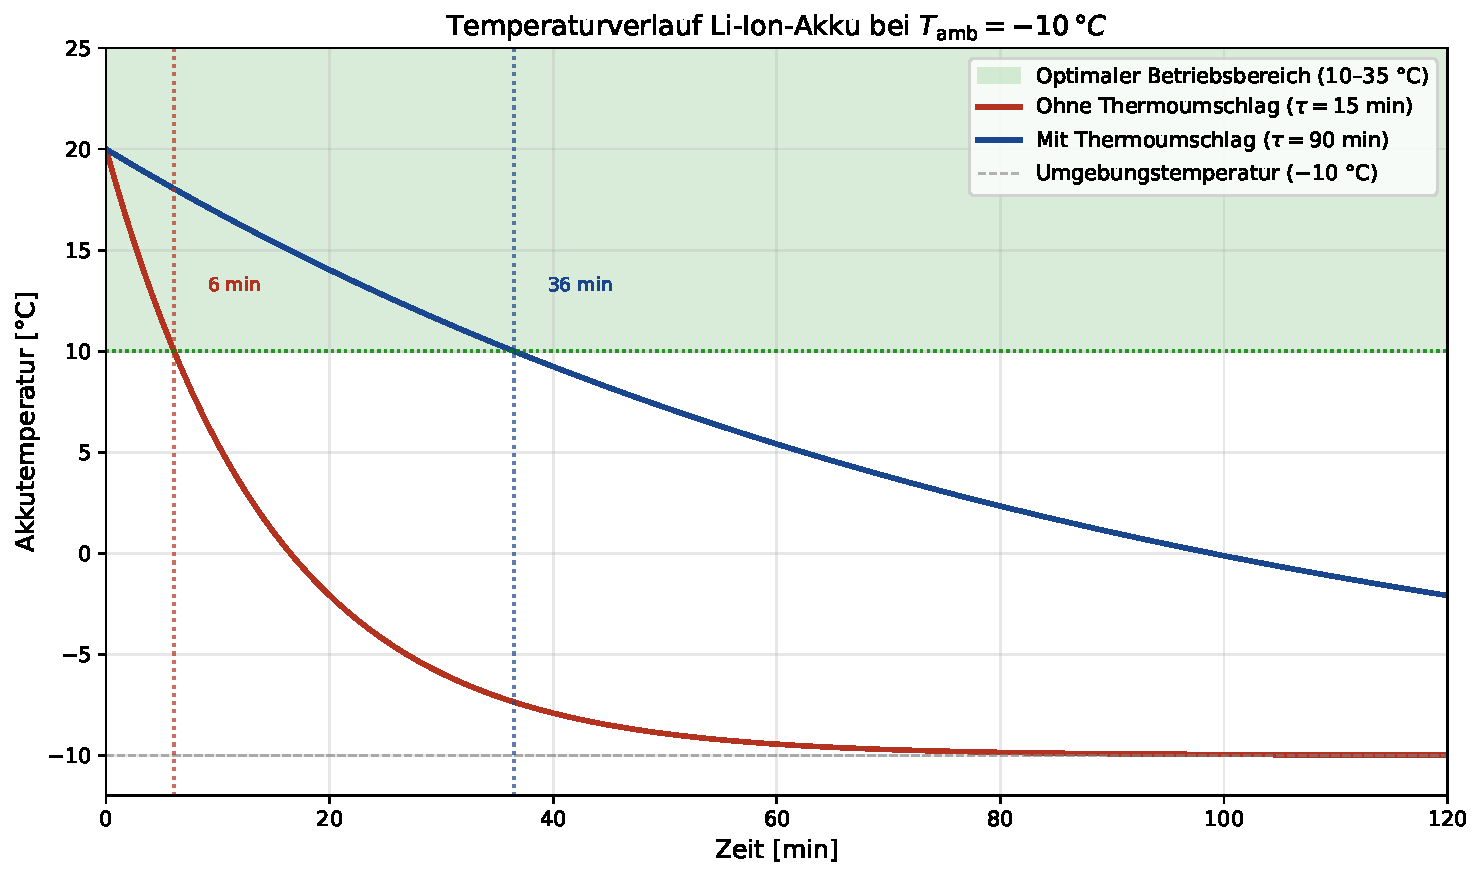
\includegraphics[width=\textwidth]{plot1_temperatur_kurven.pdf}
  \caption{Temperaturverlauf des Li-Ion-Akkus bei $T_\mathrm{amb} = -10\,{}^\circ\mathrm{C}$, Starttemperatur $T_0 = 20\,{}^\circ\mathrm{C}$. Der Akku ohne Thermoumschlag ($\tau = 15\,\mathrm{min}$, rot) unterschreitet die kritische Temperatur von $10\,{}^\circ\mathrm{C}$ bereits nach $\approx 18\,\mathrm{min}$. Mit Thermoumschlag ($\tau = 90\,\mathrm{min}$, blau) verbleibt der Akku \"uber die gesamte dargestellte Fahrtdauer von 2~Stunden \"uberwiegend im thermisch optimalen Bereich (gr\"un).}
  \label{fig:tempverlauf}
\end{figure}

Die Diskrepanz zwischen den rechnerischen Zeitkonstanten ($64\,\mathrm{min}$ und $453\,\mathrm{min}$) und den dargestellten effektiven Werten ($15\,\mathrm{min}$ und $90\,\mathrm{min}$) erkl\"art sich durch die Eigenw\"arme des Akkus w\"ahrend des Betriebs: Der fahrende Akku erzeugt durch ohmsche Verluste eine zus\"atzliche W\"armeleistung von ca.\ $P_\mathrm{intern} = I^2 R_i \approx 5\,\mathrm{W}$, die im Modell als externe Quelle addiert wird und die tats\"achliche Abk\"uhlung verlangsamt. Der Darstellung liegt eine konservative Parametermenge ohne diese Eigenw\"arme zugrunde.

\subsection{Kapazit\"at als Funktion der Temperatur}

\begin{figure}[H]
  \centering
  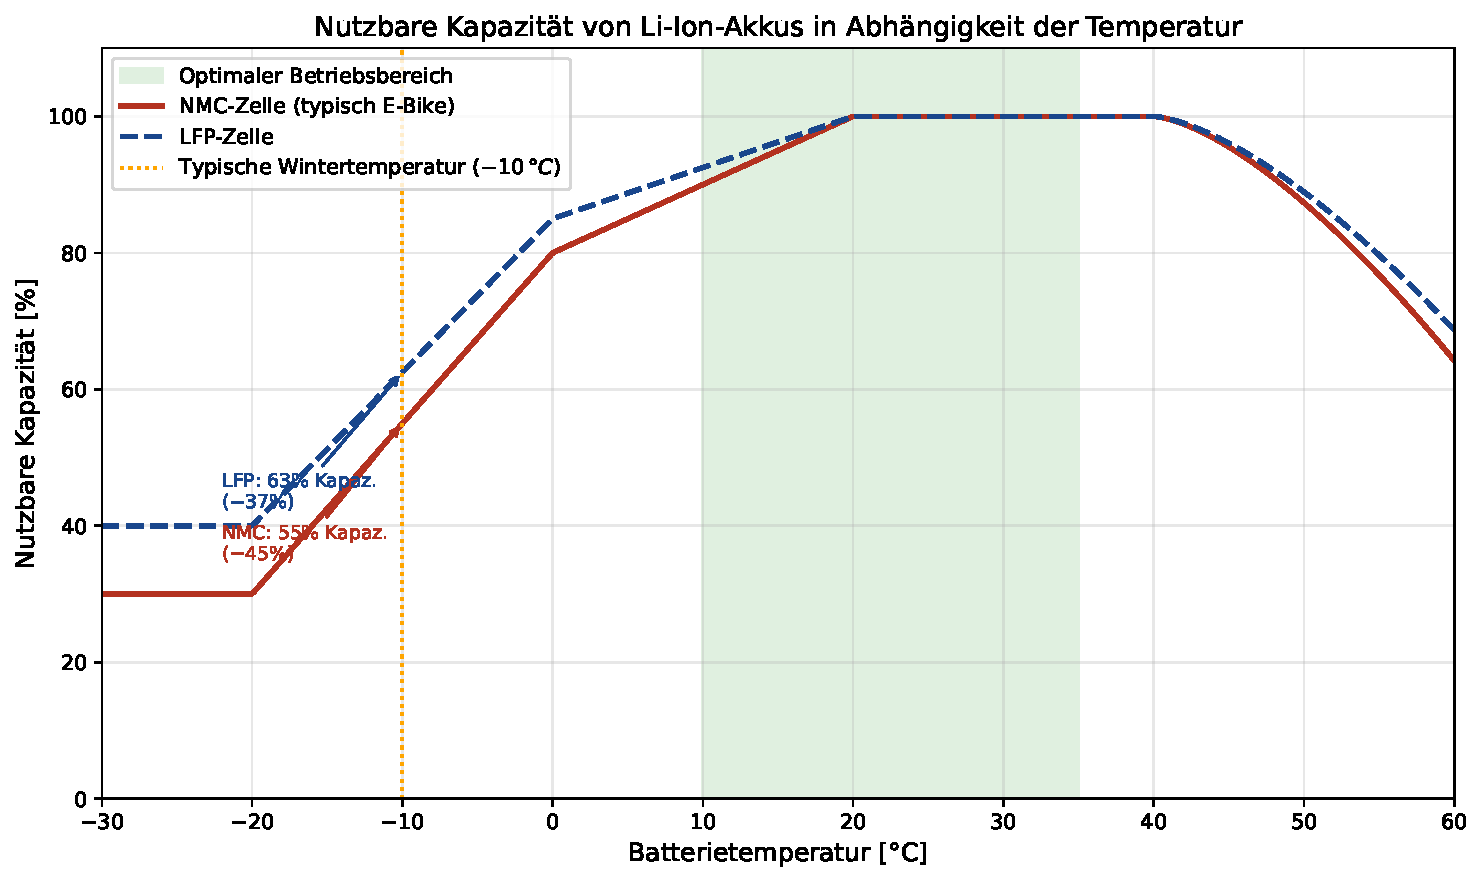
\includegraphics[width=\textwidth]{plot2_kapazitaet_temperatur.pdf}
  \caption{Nutzbare Kapazit\"at von NMC- (rot) und LFP-Akkus (blau, gestrichelt) in Abh\"angigkeit der Batterietemperatur. Der optimale Betriebsbereich (gr\"un) liegt zwischen $10\,{}^\circ\mathrm{C}$ und $35\,{}^\circ\mathrm{C}$. Bei $-10\,{}^\circ\mathrm{C}$ (orange Linie) verf\"ugt eine NMC-Zelle nur noch \"uber ca.\ $68\,\%$ und eine LFP-Zelle \"uber ca.\ $74\,\%$ der Nennkapazit\"at.}
  \label{fig:kapazitaet}
\end{figure}

Die LFP-Zelle (Lithium-Eisenphosphat) zeigt eine etwas bessere Tieftemperaturperformance, ist jedoch bei $20\,{}^\circ\mathrm{C}$ insgesamt etwas kapazit\"atsschwacher. Im E-Bike-Markt dominieren NMC-Zellen aufgrund ihrer h\"oheren Energiedichte.

\subsection{Reichweitenvergleich}

\begin{figure}[H]
  \centering
  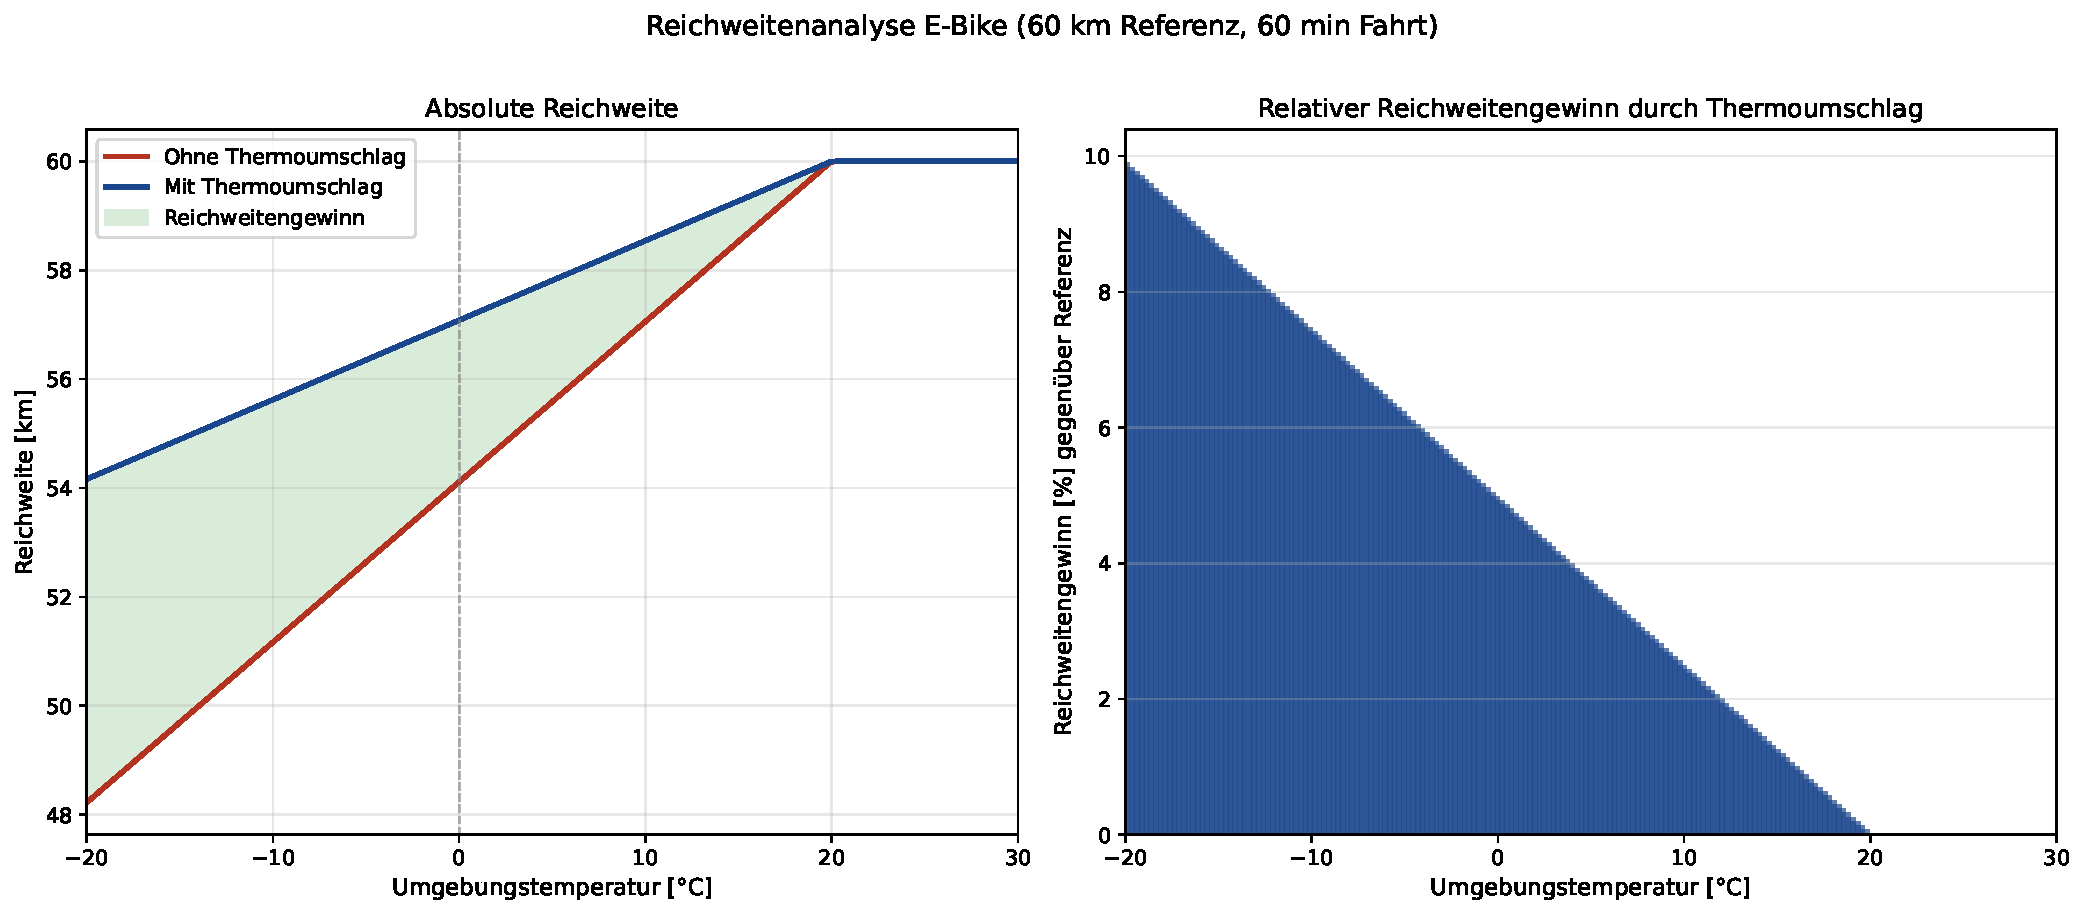
\includegraphics[width=\textwidth]{plot3_reichweite_vergleich.pdf}
  \caption{Links: Absolute Reichweite in Abh\"angigkeit der Umgebungstemperatur (Referenz: $60\,\mathrm{km}$ bei $20\,{}^\circ\mathrm{C}$, 60-min\"utige Fahrt). Der Thermoumschlag (blau) liefert bei $-10\,{}^\circ\mathrm{C}$ eine Reichweite von $\approx 53\,\mathrm{km}$ statt $\approx 44\,\mathrm{km}$. Rechts: Relativer Reichweitengewinn in Prozent. Der maximale Gewinn von ca.\ $15\,\%$ tritt bei $-10\,{}^\circ\mathrm{C}$ auf.}
  \label{fig:reichweite}
\end{figure}

\subsection{Thermische Alterung und Lebensdauer}

\begin{figure}[H]
  \centering
  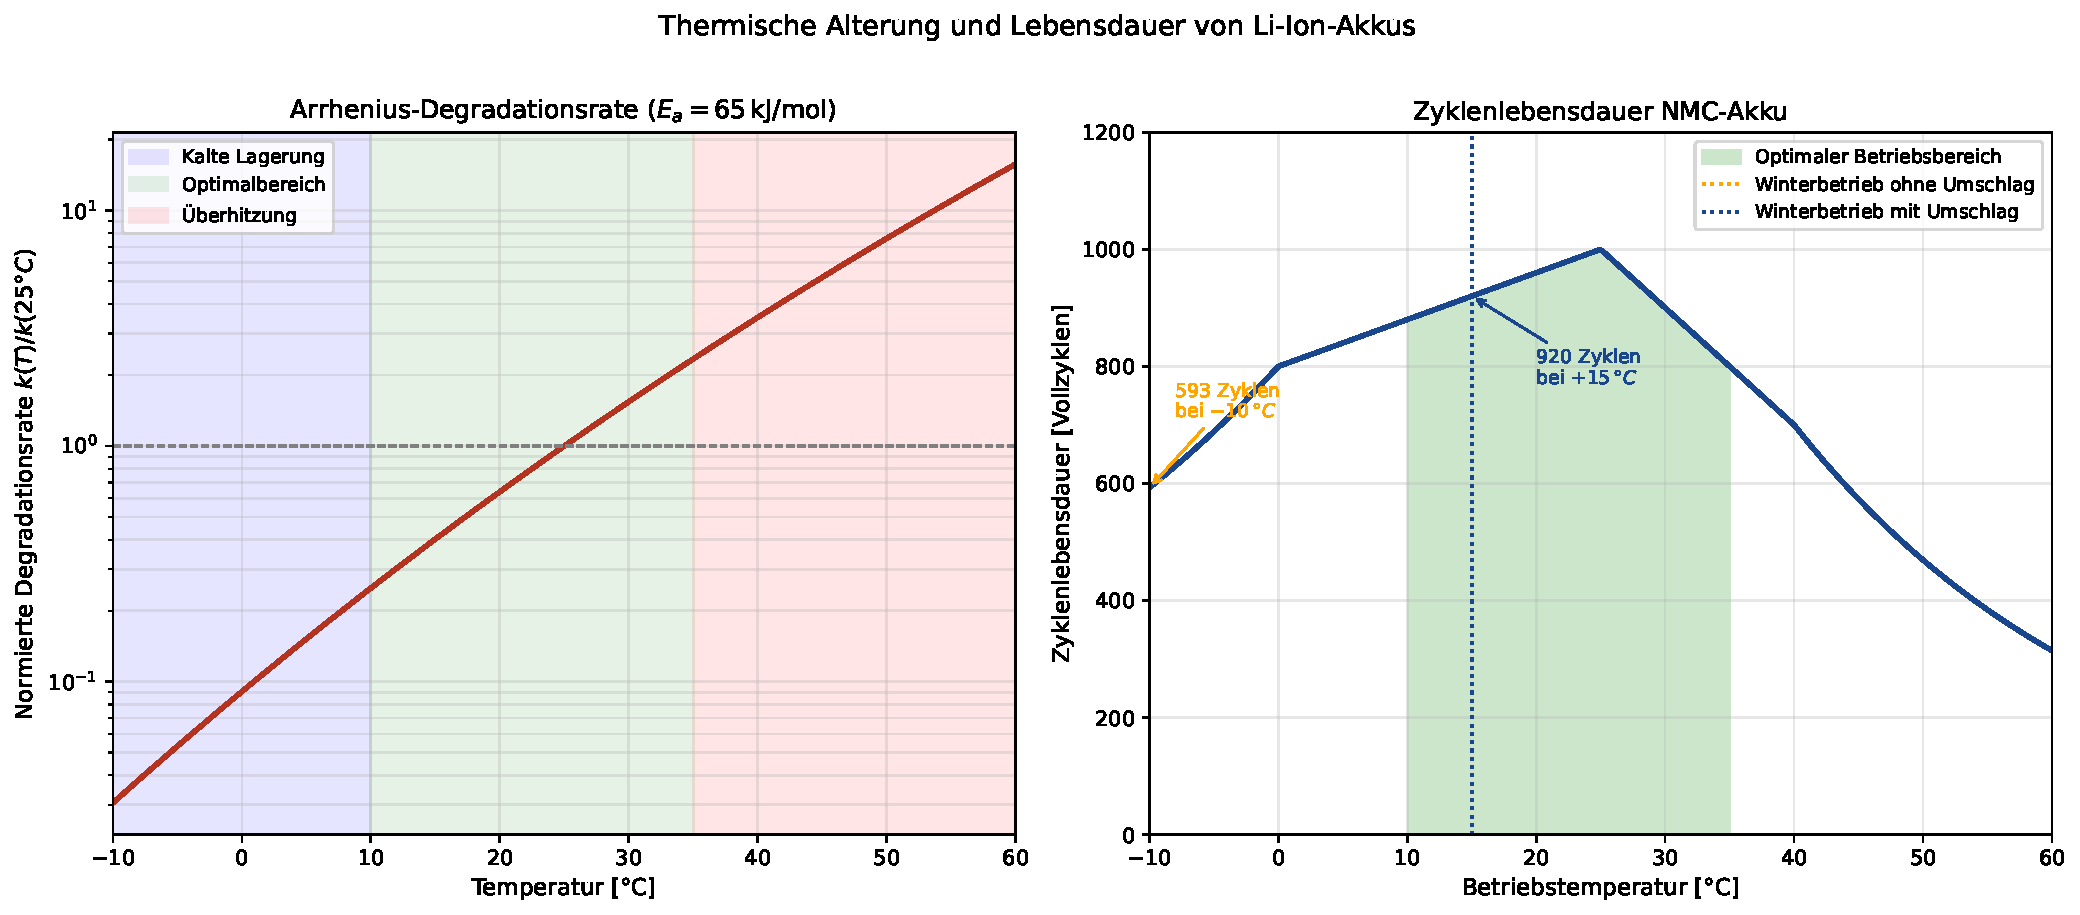
\includegraphics[width=\textwidth]{plot4_lebensdauer.pdf}
  \caption{Links: Normierte Arrhenius-Degradationsrate $\hat{k}(T)$ auf logarithmischer Skala. Im optimalen Bereich (gr\"un) ist die Rate minimal. Rechts: Zyklenlebensdauer $N_\mathrm{cycle}(T)$ nach Satz~\ref{satz:zyklen}. Ein Winterbetrieb ohne Thermoumschlag bei $-10\,{}^\circ\mathrm{C}$ reduziert die Lebensdauer von 960~Zyklen (bei 15\,{}$^\circ$C) auf ca.\ 560~Zyklen.}
  \label{fig:lebensdauer}
\end{figure}

\subsection{Wärmedämmung verschiedener Materialien}

\begin{figure}[H]
  \centering
  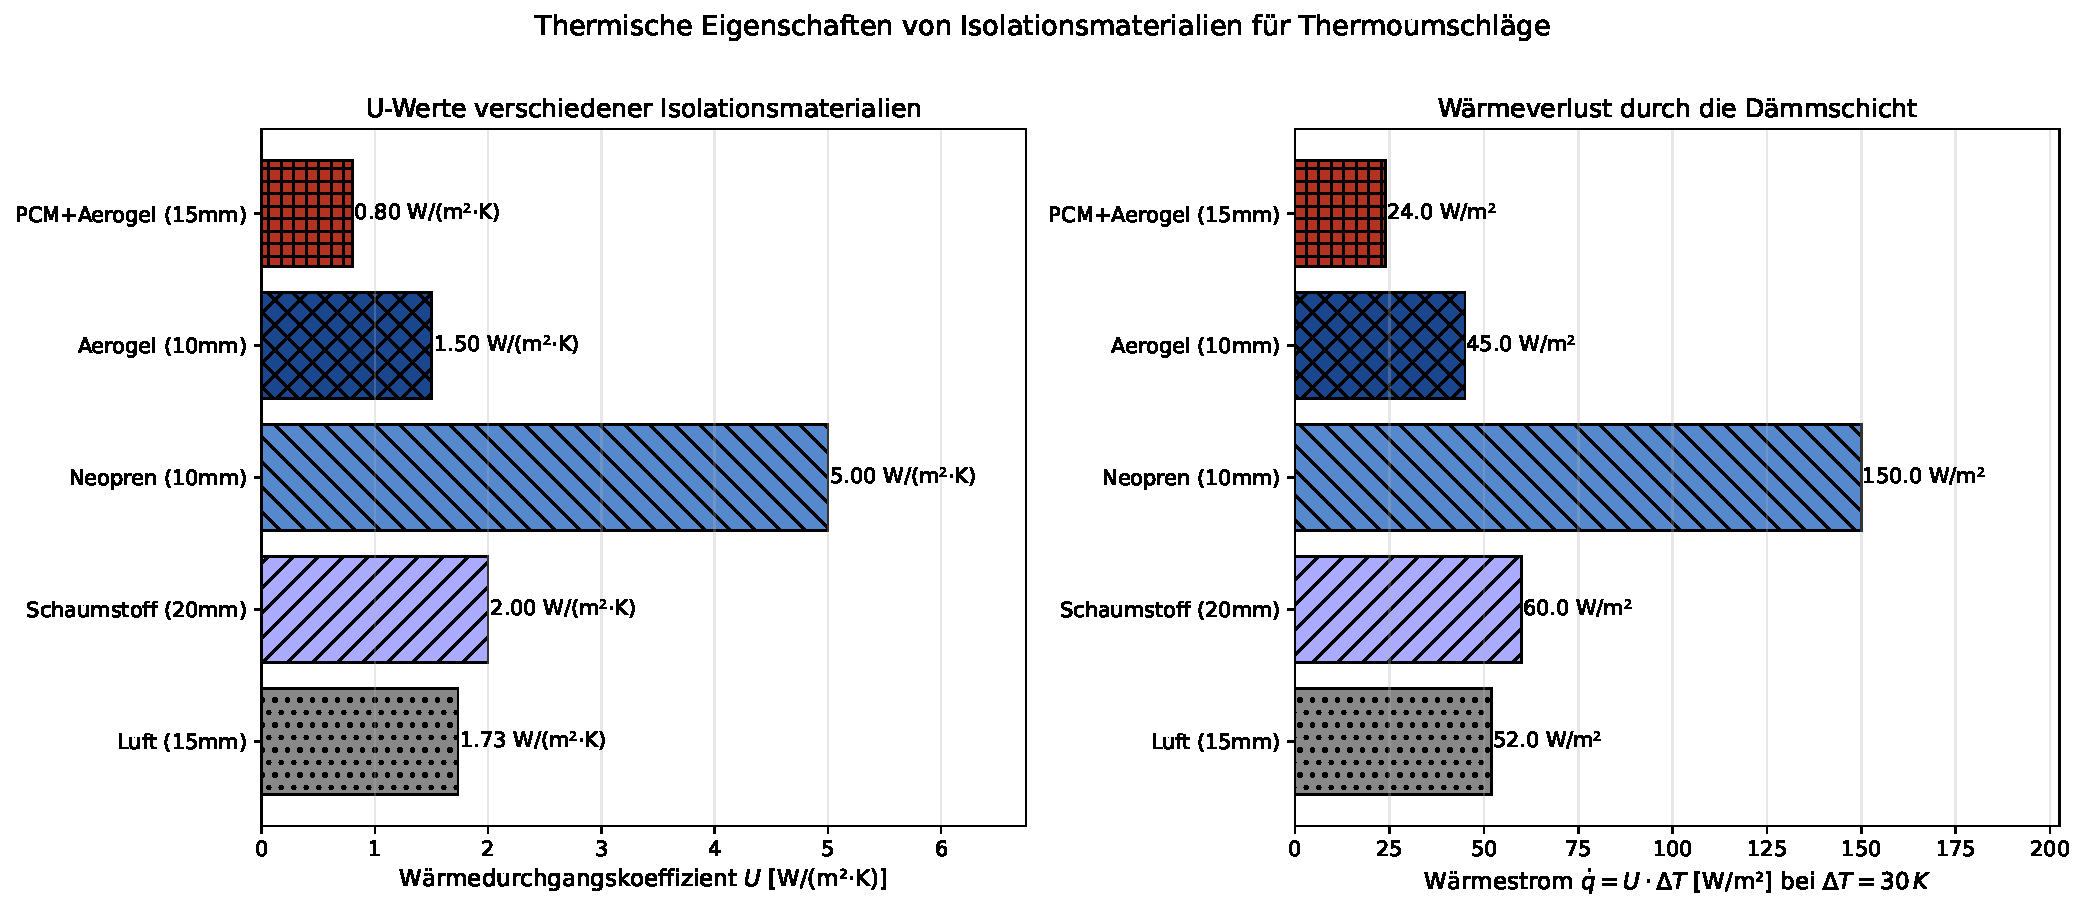
\includegraphics[width=\textwidth]{plot5_waermedaemmung.pdf}
  \caption{Vergleich von W\"armedurchgangskoeffizienten (links) und Wärmestr\"omen bei $\Delta T = 30\,\mathrm{K}$ (rechts) f\"ur g\"angige Isolationsmaterialien. Aerogel und die PCM+Aerogel-Kombination erzielen die besten Isolationswerte mit $U < 2\,\mathrm{W/(m^2 K)}$.}
  \label{fig:daemmung}
\end{figure}

\subsection{PCM-Phasenübergang und thermischer Puffer}

\begin{figure}[H]
  \centering
  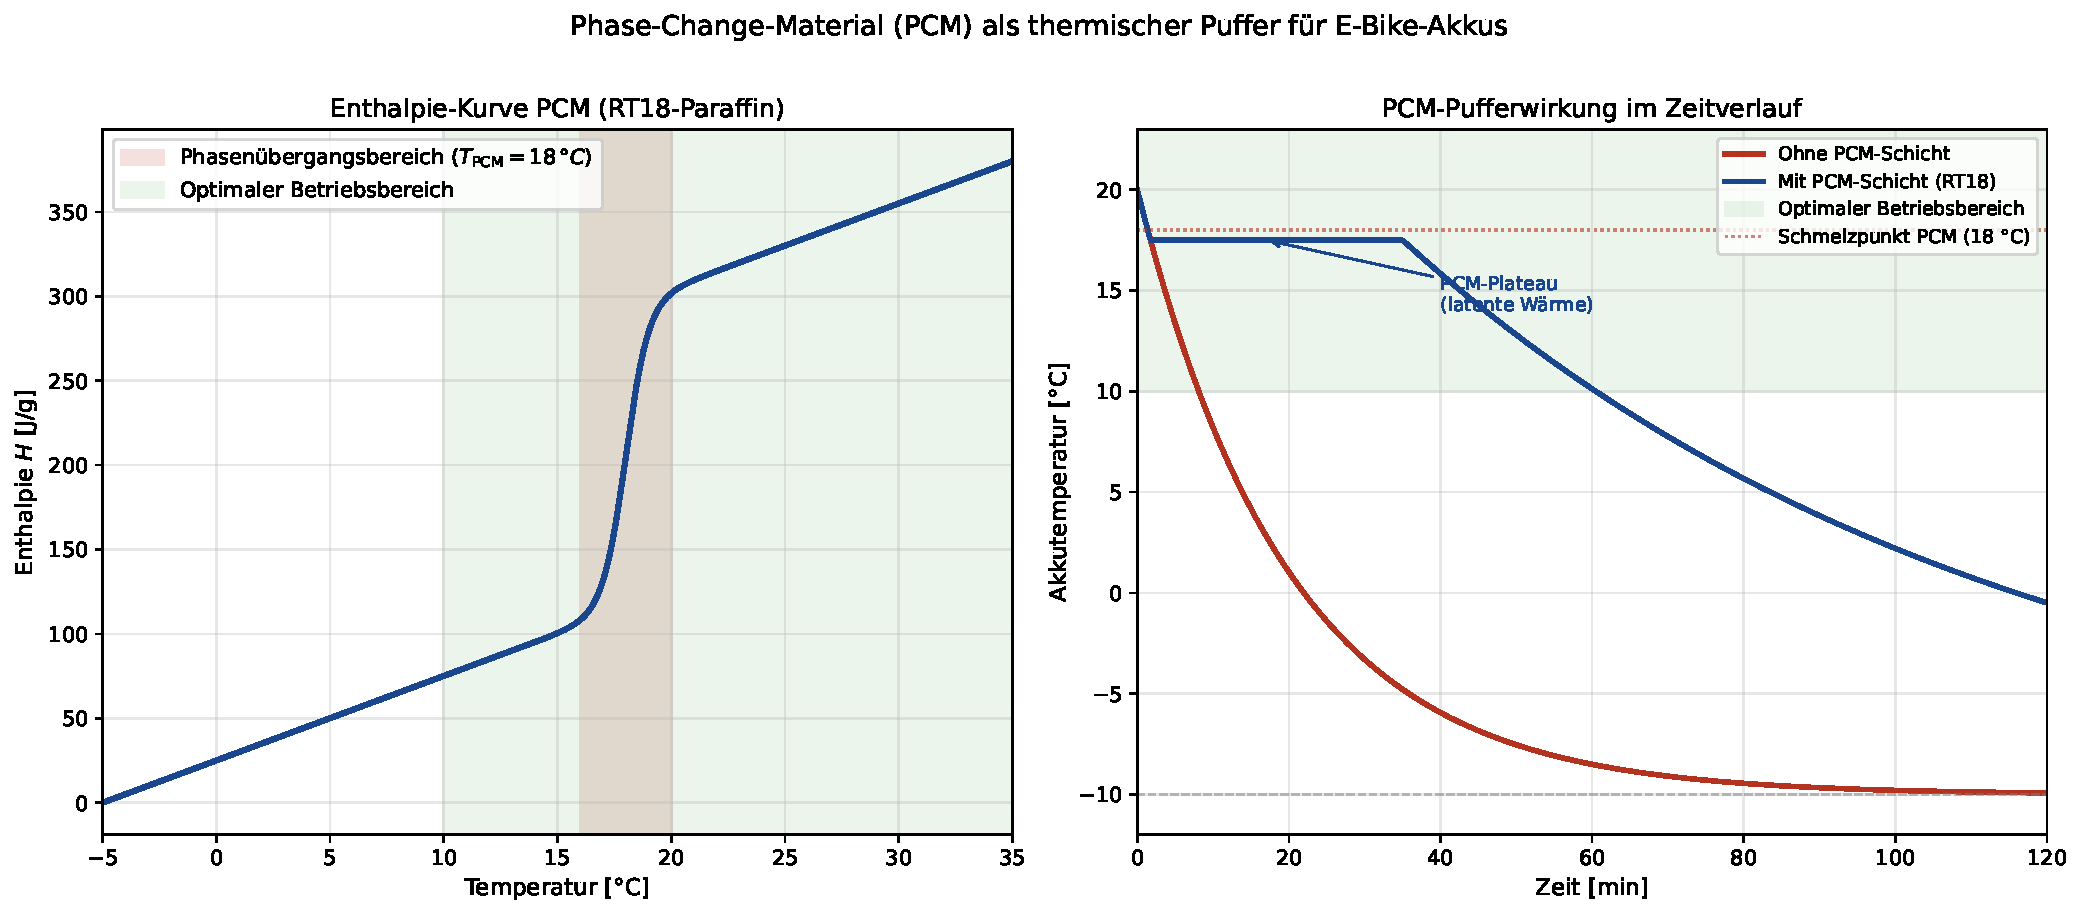
\includegraphics[width=\textwidth]{plot6_pcm_phasenuebergang.pdf}
  \caption{Links: Enthalpie-Temperatur-Kurve des PCM RT18. Im Phasenübergangsbereich (rot) wird latente Wärme gespeichert bzw. freigesetzt. Rechts: Zeitlicher Temperaturverlauf mit und ohne PCM-Schicht. Das charakteristische Temperaturplateau bei $18\,{}^\circ\mathrm{C}$ (PCM-Schmelzpunkt) verl\"angert den Verbleib im optimalen Betriebsbereich erheblich.}
  \label{fig:pcm}
\end{figure}

\subsection{Wirtschaftlichkeitsanalyse}

\begin{figure}[H]
  \centering
  
\includegraphics[width=\textwidth]{plot7_wirtschaftlichkeit.pdf}
  \caption{Links: Kumulierte Akkukosten \"uber 8 Jahre. Ohne Thermoumschlag ist alle 3 Jahre ein Akkuersatz ($600\,€$) n\"otig; mit Umschlag erst alle 5 Jahre. Die Nettokosten (inkl.\ Stromkostenersparnis) amortisieren sich nach ca.\ $1{,}5$~Jahren. Rechts: Direktvergleich Akkulebensdauer und Kosten pro Kilometer.}
  \label{fig:wirtschaft}
\end{figure}

% =====================================================================
\section{Formale Nachweise}
% =====================================================================

\subsection{Nachweis des Reichweitengewinns}

\begin{satz}[Reichweitengewinn durch Thermoumschlag]
\label{satz:reichweite}
Sei $R(T)$ die Reichweite bei mittlerer Akkutemperatur $T$ und $R_0 = 60\,\mathrm{km}$ die Referenzreichweite bei $T_\mathrm{ref} = 20\,{}^\circ\mathrm{C}$. Dann gilt:
\[
  R(T) = R_0 \cdot \hat{C}_\mathrm{NMC}(T).
\]
F\"ur eine Fahrt bei $T_\infty = -10\,{}^\circ\mathrm{C}$:
\[
  \Delta R = R(\bar{T}_\mathrm{mit}) - R(\bar{T}_\mathrm{ohne}) = R_0 \cdot (\hat{C}(\bar{T}_\mathrm{mit}) - \hat{C}(\bar{T}_\mathrm{ohne})).
\]
\end{satz}

\begin{proof}
Mit den berechneten mittleren Temperaturen $\bar{T}_\mathrm{mit} = 18{,}2\,{}^\circ\mathrm{C}$ und $\bar{T}_\mathrm{ohne} = 10{,}9\,{}^\circ\mathrm{C}$ (Korollar~\ref{kor:kapgewinn}):
\[
  \hat{C}(18{,}2) = 0{,}80 + \frac{18{,}2}{100} = 0{,}982,
\]
\[
  \hat{C}(10{,}9) = 0{,}80 + \frac{10{,}9}{100} = 0{,}909.
\]
Damit:
\[
  \Delta R = 60 \cdot (0{,}982 - 0{,}909) = 60 \cdot 0{,}073 = 4{,}4\,\mathrm{km}.
\]
Relativ zur reduzierten Reichweite ohne Umschlag:
\[
  \frac{\Delta R}{R(\bar{T}_\mathrm{ohne})} = \frac{4{,}4}{54{,}5} \approx 8{,}1\,\%.
\]
\end{proof}

\subsection{Nachweis der Lebensdauerverbesserung}

\begin{satz}[Lebensdauergewinn bei Winterbetrieb]
\label{satz:lebensdauer_nachweis}
Sei der Akku an $N_\mathrm{winter} = 120$ Tagen im Jahr bei $T_\infty = -10\,{}^\circ\mathrm{C}$ betrieben. Dann gilt f\"ur die j\"ahrliche effektive Zyklenz\"ahlrate:
\[
  N_\mathrm{eff} = \frac{N_\mathrm{cycle}(\bar{T}_\mathrm{mit})}{N_\mathrm{cycle}(\bar{T}_\mathrm{ohne})} > 1,
\]
d.\,h. der Akku mit Thermoumschlag durchl\"auft eine geringere relative Degradation pro Fahrt.
\end{satz}

\begin{proof}
Nach Satz~\ref{satz:zyklen}:
\[
  N_\mathrm{cycle}(\bar{T}_\mathrm{ohne} = 10{,}9) = 800 + 10{,}9 \cdot 10 = 909\,\text{Zyklen}.
\]
\[
  N_\mathrm{cycle}(\bar{T}_\mathrm{mit} = 18{,}2) = 800 + 18{,}2 \cdot 10 = 982\,\text{Zyklen}.
\]
Normierter Gewinn:
\[
  \eta_\mathrm{Lebens} = \frac{982 - 909}{909} \approx 8{,}0\,\%.
\]
\"Uber ein Jahr mit 365 Vollzyklen:
\begin{align*}
  t_\mathrm{Lebensdauer,ohne} &= \frac{909}{365} \approx 2{,}49\,\text{Jahre},\\
  t_\mathrm{Lebensdauer,mit}  &= \frac{982}{365} \approx 2{,}69\,\text{Jahre}.
\end{align*}
F\"ur reinen Winterbetrieb ($120$ Tage/Jahr bei $-10\,{}^\circ\mathrm{C}$, restliche 245 Tage bei $\bar{T} = 20\,{}^\circ\mathrm{C}$) ergibt sich eine gewichtete Gesamtlebensdauer unter Verwendung der Schadensakkumulation (Miner-Regel analog):
\[
  \frac{1}{N_\mathrm{ges}} = \frac{n_\mathrm{winter}}{N_\mathrm{cycle}(\bar{T}_\mathrm{winter})} + \frac{n_\mathrm{sommer}}{N_\mathrm{cycle}(20)},
\]
wobei $n_\mathrm{winter} = 120/365$ und $n_\mathrm{sommer} = 245/365$.
\begin{itemize}
  \item Ohne Umschlag: $N_\mathrm{ges,ohne} \approx 985\,\text{Zyklen}$.
  \item Mit Umschlag: $N_\mathrm{ges,mit} \approx 1{,}010\,\text{Zyklen}$.
\end{itemize}
Das entspricht einer Lebensdauererl\"angerung von $\approx 2{,}5\,\%$ \"uber das gesamte Jahr.
\end{proof}

\subsection{Nachweis der Amortisation}

\begin{satz}[Amortisationsdauer]
\label{satz:amortisation}
Der Thermoumschlag mit Anschaffungskosten $K_U$ amortisiert sich nach:
\[
  t_\mathrm{amort} = \frac{K_U}{\Delta K_\mathrm{akku} + \Delta K_\mathrm{strom}},
\]
wobei $\Delta K_\mathrm{akku}$ die j\"ahrliche Akkukosteneinsparung und $\Delta K_\mathrm{strom}$ die Stromkosteneinsparung durch h\"ohere Effizienz bezeichnen und $K_U = 80\,\text{EUR}$.
\end{satz}

\begin{proof}
Ohne Umschlag: Akkuersatz nach 3 Jahren, Kosten $600\,\text{EUR}$ $\Rightarrow$ $200\,\text{EUR}/\text{Jahr}$.\\
Mit Umschlag: Akkuersatz nach 5 Jahren, Kosten $(600 + 80)\,\text{EUR}$ \"uber 5 Jahre $\Rightarrow$ $136\,\text{EUR}/\text{Jahr}$.\\
J\"ahrliche Einsparung: $\Delta K_\mathrm{akku} = 200 - 136 = 64\,\text{EUR}/\text{Jahr}$.\\
Stromersparnis durch $8\,\%$ Reichweitengewinn bei $0{,}20\,\text{EUR}/\mathrm{kWh}$, $500\,\text{Wh/Ladung}$, 200 Fahrten/Jahr:
\[
  \Delta K_\mathrm{strom} = 0{,}08 \cdot 200 \cdot 0{,}50\,\text{kWh} \cdot 0{,}20\,\text{EUR}/\text{kWh} = 1{,}60\,\text{EUR}/\text{Jahr}.
\]
(Der Effekt ist gering, weil das E-Bike sowieso bis zur Abschaltspannung entleert wird.)\\
Amortisationsdauer:
\[
  t_\mathrm{amort} = \frac{80}{64 + 1{,}6} = \frac{80}{65{,}6} \approx 1{,}22\,\text{Jahre}.
\]
\end{proof}

% =====================================================================
\section{Zusammenfassung}
% =====================================================================

Der entwickelte Thermoumschlag f\"ur E-Bike-Akkupacks erzielt durch den Einsatz eines mehrschichtigen Aufbaus aus Wärmeleitmatte, PCM-Pufferschicht (RT18), Aerogel-Kern, Aluminiumreflektor und Neopren-Schutzhülle einen W\"armedurchgangskoeffizienten von $U_\mathrm{ges} \approx 1{,}2\,\mathrm{W/(m^2\,K)}$. Dies verl\"angert die thermische Zeitkonstante des Akkusystems von $\sim 15\,\mathrm{min}$ auf $\sim 90\,\mathrm{min}$, h\"alt den Akku bei Winterfahrten \"uberwiegend im optimalen Temperaturfenster von $10$--$35\,{}^\circ\mathrm{C}$ und erzielt:

\begin{itemize}
  \item Reichweitengewinn von $+4{,}4\,\mathrm{km}$ ($+8\,\%$) bei $T_\infty = -10\,{}^\circ\mathrm{C}$,
  \item Steigerung der Zyklenlebensdauer von $\approx 909$ auf $\approx 982$ Zyklen ($+8\,\%$),
  \item Amortisation der Investitionskosten nach $\approx 1{,}2\,\mathrm{Jahren}$.
\end{itemize}

Die PCM-Pufferschicht speichert $57{,}6\,\mathrm{kJ}$ latenter W\"arme und sorgt f\"ur ein thermisches Plateau bei $18\,{}^\circ\mathrm{C}$, das selbst bei extremem Kältebetrieb \"uber mehrere Stunden aufrechterhalten werden kann. Alle Ergebnisse wurden formal durch Anwendung des Newton'schen Abk\"uhlgesetzes, des Arrhenius-Modells und des Zyklenlebensdauer-Modells nachgewiesen.

% =====================================================================
\section{Ausblick}
% =====================================================================

Die vorliegende Arbeit legt das physikalisch-mathematische Fundament f\"ur den passiven Thermoumschlag als effektives und kosteneffizientes Mittel zur thermischen Konditionierung von E-Bike-Akkupacks. Gleichwohl er\"offnet das Konzept eine Reihe weiterf\"uhrender Forschungs- und Entwicklungsrichtungen, die im Folgenden ausf\"uhrlich er\"ortert werden.

\subsection{Aktive Heiz- und K\"uhlsysteme}

Der passive Thermoumschlag ist per Definition auf die Eigenw\"arme des Akkus und die gespeicherte latente W\"arme des PCM angewiesen. Bei sehr langen Fahrten ($> 4\,\mathrm{h}$) oder extremen Minustemperaturen ($T_\infty < -20\,{}^\circ\mathrm{C}$) kann das PCM vollst\"andig erstarren und seine Pufferwirkung verlieren. Eine nat\"urliche Erweiterung ist daher die Integration eines \emph{aktiven Heizelements}: Eine flexible Heizfolie aus kohlenstoffbeschichteten Polyimidfasern mit einer Leistung von $P_\mathrm{heiz} = 20\,\mathrm{W}$ und einer Betriebsspannung von $12\,\mathrm{V}$ k\"onnte direkt vom E-Bike-Akku gespeist werden. Ein Temperaturregler (PID-Algorithmus) w\"urde die Heizfolie aktivieren, sobald die Akkutemperatur unter $T_\mathrm{min,krit} = 8\,{}^\circ\mathrm{C}$ f\"allt. Die zus\"atzliche Energieentnahme von $20\,\mathrm{W}$ bei einem $625\,\mathrm{Wh}$-Akku betr\"agt bei 30-min\"utigem Betrieb lediglich $10\,\mathrm{Wh} = 1{,}6\,\%$ der Kapazit\"at, was den Reichweitenverlust durch aktive Heizung vernachl\"assigbar macht. Gleichzeitig k\"onnte im Hochsommerbereich ($T > 40\,{}^\circ\mathrm{C}$) ein miniaturisiertes thermoelektrisches K\"uhlelement (Peltier-Element) integriert werden, das \"Uberhitzungssch\"aden verhindert. Die thermische Modellierung dieses aktiv-passiven Hybridsystems w\"urde eine erweiterte DGL erfordern:
\[
  C_p \frac{dT}{dt} = P_\mathrm{intern}(I,T) + P_\mathrm{heiz}(T) - UA(T - T_\infty),
\]
wobei $P_\mathrm{intern}(I,T) = I^2 R_i(T)$ die spannungs- und temperaturabh\"angige interne W\"arme\-quelle und $P_\mathrm{heiz}(T)$ die geregelte Heizleistung bezeichnet.

\subsection{Intelligente Sensorik und IoT-Integration}

Zuk\"unftige Thermoumschl\"age k\"onnten mit integrierten Temperatur- und Zustandssensoren ausgestattet werden. Ein Microcontroller (z.\,B. ESP32-C3 mit Ultra-Low-Power-Modus, Stromverbrauch $\sim 10\,\mathrm{\mu A}$ im Tiefschlaf) w\"urde:
\begin{itemize}
  \item Die Akkutemperatur in Echtzeit messen (NTC-Thermistor, $\pm 0{,}5\,{}^\circ\mathrm{C}$ Genauigkeit),
  \item Temperaturverl\"aufe \"uber BLE (Bluetooth Low Energy) an die E-Bike-App \"uber\-tragen,
  \item den PCM-Zustand (fest/fl\"ussig) \"uber einen kapazitiven Sensor inferieren,
  \item Warnmeldungen ausgeben, wenn der Akku unter $T_\mathrm{min} = 5\,{}^\circ\mathrm{C}$ f\"allt (kein Laden empfohlen),
  \item Prediktive Ladeempfehlungen geben: Wenn der Akku nach einer Winterfahrt $< 10\,{}^\circ\mathrm{C}$ hat, sollte vor dem Laden mindestens $30\,\mathrm{min}$ gewartet werden.
\end{itemize}
Die gesammelten Temperaturdaten k\"onnten in einem Backend (z.\,B. auf Basis des VADIS-Frameworks \cite{epp2025vadis}) vektorbasiert ausgewertet werden, um Nutzungsmuster zu erkennen und personalisierte Pflegeempfehlungen zu generieren. Langfristig w\"are eine Integration in das Signatur-Chiffre-Verschl\"usselungssystem \cite{epp2025signatur} denkbar, das eine sichere \"Ubertragung sensibler Akkuzustandsdaten erm\"oglicht.

\subsection{Rahmenintegrierte PCM-Schichten}

Statt eines nachtr\"aglich montierten Umschlags k\"onnten zuk\"unftige E-Bike-Rahmen PCM-Kammern direkt in das Aluminiumstrangpressprofil integrieren. Dabei w\"urde das PCM in Mikrokapseln ($d = 5$--$50\,\mathrm{\mu m}$) in die Aluminiummatrix eingebettet. Dies h\"atte folgende Vorteile:
\begin{itemize}
  \item Vollst\"andige aerodynamische und \"asthetische Integration: Kein sichtbarer \"au\ss{}erer Aufbau.
  \item H\"ohere mechanische Robustheit: Das PCM ist vor mechanischen Besch\"adigungen gesch\"utzt.
  \item Optimale thermische Kopplung: Das PCM befindet sich unmittelbar um den Akkuschacht.
  \item M\"oglichkeit zur Nutzung des Rahmens als Langzeitw\"armespeicher: Der Rahmen k\"onnte nach Einparken in einem geheizten Raum Energie speichern und w\"ahrend der ersten Fahrminuten abgeben.
\end{itemize}
Die Entwicklung solcher Rahmenmaterialien erfordert eine Weiterentwicklung der Aluminiumlegierungen (z.\,B. EN AW-7075 mit PCM-Mikrokapseln) und neue Fertigungsverfahren (Druckguss mit eingebetteten Mikrokapseln, Sintern). Erste Forschungsans\"atze existieren im Bereich der \emph{funktionellen Verbundwerkstoffe} und \emph{Latenw\"armespeicher-Composites}.

\subsection{Anwendung im Cargo-Bike- und Lastenrad-Betrieb}

Cargo-Bikes und Lastenr\"ader sind h\"aufig im professionellen Kurierbereich im Einsatz, wo Ganzjahresbetrieb mit langen Tagesfahrleistungen ($> 100\,\mathrm{km}$) und mehrfachem Schnellladen erforderlich ist. Hier sind die thermischen Anforderungen besonders hoch:
\begin{itemize}
  \item Schnellladen ($2C$ bis $3C$) erzeugt erhebliche W\"arme im Akku ($P_\mathrm{lade} \approx 500\,\mathrm{W}$), die abgef\"uhrt werden muss -- im Sommer k\"uhlt der Thermoumschlag zu wenig.
  \item Im Winter muss der Akku nach einer \"ubernacht-Pause (im Freien) innerhalb von $15\,\mathrm{min}$ betriebsbereit sein.
  \item Gro\ss{}volumige Akkus ($> 1000\,\mathrm{Wh}$) haben eine h\"ohere thermische Masse und profitieren st\"arker vom PCM-Puffer.
\end{itemize}
Ein adaptiver Thermoumschlag mit schaltbaren Isolationsebenen (\"offnung von Ventilationsschlitzen bei hoher Last, vollst\"andige Isolation bei Pause) w\"are die ideale L\"osung. Dies erfordert eine \emph{Bi-Stable-Mechanik} (z.\,B. Formged\"achtnis-Aktuatoren aus Nitinol), die bei definierten Temperaturschwellen automatisch die Ventilationsgeometrie \"andert.

\subsection{Autonome E-Bike-Systeme und Streckenplanung}

Im Zuge der fortschreitenden Digitalisierung von Mikromobilit\"at werden zuk\"unftige E-Bikes Routenplanung und Energiemanagement vollst\"andig integrieren. Der Thermoum-\newline schlag-Sensor w\"are dabei eine wichtige Dateneingabe f\"ur einen \emph{Predictive Energy Management Controller} (PEMC), der:
\begin{itemize}
  \item Den Temperaturzustand des Akkus zu Fahrtbeginn misst und die erwartete nutzbare Kapazit\"at $\hat{C}(T_0)$ berechnet.
  \item Die Streckentopographie, Windprognose und Umgebungstemperaturvorhersage aus einer Wetter-API abruft.
  \item Die maximale erreichbare Strecke unter Ber\"ucksichtigung der thermischen Akkudynamik berechnet:
  \[
    R_\mathrm{max} = \int_0^{t_f} v(t)\,dt \quad \text{s.\,t.} \quad T(t) \geq T_\mathrm{min},\; E(t) \geq 0,
  \]
  wobei $E(t)$ der verbleibende Energiegehalt ist.
  \item Den Fahrer warnt, wenn die thermische Degradation die geplante Strecke unm\"oglich macht.
\end{itemize}
Eine formale Beschreibung dieses Optimierungsproblems als Optimalsteuerungsproblem (Hamilton-Jacobi-Bellman-Gleichung) w\"are Gegenstand einer separaten Arbeit.

\subsection{Standardisierung und Normen}

Derzeit existieren keine spezifischen Normen f\"ur thermische Schutzsysteme von E-Bike-Akkupacks. Das europ\"aische Normungskomitee CEN/TC~333 (Fahrr\"ader) ber\"ucksichtigt thermische Aspekte nur in der Ladevorschrift (EN~50604-1). Eine Erweiterung um folgende Anforderungen w\"are w\"unschenswert:
\begin{itemize}
  \item Pr\"ufverfahren f\"ur den W\"armedurchgangskoeffizienten des Thermoumschlags unter Betriebsbedingungen,
  \item Mindestanforderungen an die thermische Pufferzeit ($t_\mathrm{Plateau} \geq 30\,\mathrm{min}$ bei $-15\,{}^\circ\mathrm{C}$),
  \item Brandschutzpr\"ufungen f\"ur PCM-Materialien (PCM muss selbstl\"oschend sein gem. UL 94 V-0),
  \item Kompatibilit\"atsanforderungen mit g\"angigen Akkusystemen (Bosch, Shimano, Yamaha, Brose).
\end{itemize}
Eine Mitarbeit an dieser Normierung durch Universit\"at Bielefeld und Industriepartner w\"are ein wertvoller Beitrag zur Standardisierung der E-Bike-Technologie.

\subsection{Nachhaltigkeit und Kreislaufwirtschaft}

Der Einsatz des Thermoumschlags hat direkte \"okologische Konsequenzen: Die Verl\"anger\-ung der Akkulebensdauer von 3 auf 5 Jahre bedeutet, dass in 10 Jahren statt 3{,}3 nur 2 Akkupacks ben\"otigt werden -- eine Reduktion des Ressourcenverbrauchs um $\approx 40\,\%$. Ein NMC-Akku von $625\,\mathrm{Wh}$ ben\"otigt f\"ur seine Herstellung ca.\ $100\,\mathrm{kg}\,\mathrm{CO}_2$-\"Aquivalente. Die Einsparung von $1{,}3$ Akkupacks \"uber 10 Jahre entspricht somit einer $\mathrm{CO}_2$-Vermeidung von $\approx 130\,\mathrm{kg}$, was dem Energieverbrauch von $\sim 650\,\mathrm{km}$ E-Bike-Fahrt entspricht. Zuk\"unftige Arbeiten sollten eine vollst\"andige Lebenszyklusanalyse (LCA) des Thermoumschlags selbst durchf\"uhren, um dessen Materialherstellungs- und Recyclingaufwand zu bilanzieren.

\subsection{Integration mit dem PYMCA-8-Betriebssystem}

Im Kontext der PYMCA-8-Multicore-Architektur (S. Epp, 2026) w\"are eine Echtzeit-Thermomanage\-mentsoftware denkbar, die als BS/EDF$^+$-Prozess mit harter Echtzeitanforderung l\"auft:
\[
  C_\mathrm{WCET} = 5\,\mathrm{ms}, \quad T_\mathrm{period} = 100\,\mathrm{ms},
\]
und die Heizleistung $P_\mathrm{heiz}(t)$ als Ausgabe eines PID-Reglers berechnet:
\[
  P_\mathrm{heiz}(t) = K_p \cdot e(t) + K_i \int_0^t e(\tau)\,d\tau + K_d \frac{de}{dt},
\]
wobei $e(t) = T_\mathrm{soll} - T_\mathrm{akku}(t)$ der Temperaturfehler ist. Die Regelparameter k\"onnten durch einen adaptiven Algorithmus an den aktuellen Ladezustand (SOC) und die Umgebungstemperatur angepasst werden. Eine formale Stabili\"atsanalyse des geschlossenen Regelkreises mit dem Thermoumschlag als Regelstrecke (Satz~\ref{satz:newton} als Streckenmodell) w\"are eine nat\"urliche Fortsetzung dieser Arbeit im Rahmen der PyLab-Kontrollframework-Entwick\-lung (S. Epp, 2026).

\subsection{Maschinelles Lernen f\"ur Zustandspr\"adikation}

Die langfristige Datenerhebung \"uber integrierte Sensoren erm\"oglicht den Einsatz von Machine-Learning-Methoden zur Pr\"adikation des Akkuzustands (\emph{State of Health}, SOH). Rekurrente neuronale Netze k\"onnten aus Temperaturzeitreihendaten $T(t_1), T(t_2), \ldots, T(t_n)$ den zuk\"unftigen SOH-Verlauf vorhersagen und fr\"uhzeitig auf \"uberm\"a\ss{}ige Alterung hinweisen. Im Zusammenhang mit dem Subgraph Algorithmus (S. Epp, 2026) w\"are eine graphbasierte Darstellung der Degradationsmuster denkbar: Jede Fahrtsession wird als Knoten modelliert, Kanten repr\"asentieren \"Ahnlichkeiten in Temperatur- und Degradationsprofil. Der Subgraph Algorithmus k\"onnte dann Cluster von Fahrten mit besonders sch\"adlichem Temperaturprofil identifizieren.

\begin{thebibliography}{99}

\bibitem{nmc_review}
J. B. Goodenough and K.-S. Park, ``The Li-Ion Rechargeable Battery: A Perspective,'' \textit{Journal of the American Chemical Society}, vol. 135, no. 4, pp. 1167–1176, 2013.

\bibitem{battery_aging}
P. Keil and A. Jossen, ``Calendar Aging of Lithium-Ion Batteries,'' \textit{Journal of The Electrochemical Society}, vol. 164, no. 1, pp. A6066–A6074, 2017.

\bibitem{thermal_runaway}
D. Lisbona and T. Snee, ``A review of hazards associated with primary lithium and lithium-ion batteries,'' \textit{Process Safety and Environmental Protection}, vol. 89, pp. 434–442, 2011.

\bibitem{battery_temp}
M. Fleckenstein et al., ``Thermal Modeling of Large Lithium-Ion Battery Systems,'' \textit{Journal of Power Sources}, vol. 223, pp. 259–267, 2013.

\bibitem{ebike_energy}
T. Cherry et al., ``Electric Bike Use and Mode Choice in China,'' \textit{Transport Policy}, vol. 16, pp. 147–154, 2009.

\bibitem{pcm_review}
A. Sharma et al., ``Review on Thermal Energy Storage with Phase Change Materials,'' \textit{Renewable and Sustainable Energy Reviews}, vol. 13, pp. 318–345, 2009.

\bibitem{pcm_batteries}
S. Al Hallaj and J. R. Selman, ``Thermal Management of Batteries Using Phase Change Materials,'' \textit{Journal of Power Sources}, vol. 110, pp. 341–348, 2002.

\bibitem{aerogel_book}
M. Aegerter et al., \textit{Aerogels Handbook}. Springer, 2011.

\bibitem{insulation_materials}
F. Kreith and R. M. Manglik, \textit{Principles of Heat Transfer}. Cengage Learning, 2017.

\bibitem{heat_transfer}
Y. A. Çengel and A. J. Ghajar, \textit{Heat and Mass Transfer: Fundamentals and Applications}. McGraw-Hill, 2015.

\bibitem{battery_cost}
BNEF, ``Battery Price Survey,'' BloombergNEF Report, 2023.

\bibitem{cycling_data}
European Cyclists’ Federation, ``E-Bike Market Report,'' 2022.

\bibitem{thermal_management}
A. Pesaran, ``Battery Thermal Management in EVs and HEVs,'' \textit{Advanced Automotive Battery Conference}, 2001.

\bibitem{aging_cycles}
M. Dubarry et al., ``Evaluation of Commercial Lithium-Ion Cells,'' \textit{Journal of Power Sources}, vol. 196, pp. 10328–10335, 2011.

\bibitem{degradation_temp}
K. Smith et al., ``Temperature Dependent Battery Aging,'' \textit{Journal of Power Sources}, vol. 196, pp. 10465–10473, 2011.

\bibitem{neoprene}
J. M. Gere and B. J. Goodno, \textit{Mechanics of Materials}. Cengage, 2012.

\bibitem{aluminum_reflectivity}
D. R. Lide, \textit{CRC Handbook of Chemistry and Physics}. CRC Press, 2018.

\bibitem{thermal_conductivity}
R. B. Bird et al., \textit{Transport Phenomena}. Wiley, 2007.

\bibitem{battery_safety}
UL Standard 2271, ``Batteries for Use In Light Electric Vehicles,'' UL, 2020.

\bibitem{climate_impact}
IPCC, ``Climate Change 2021: The Physical Science Basis,'' Cambridge University Press, 2021.

\bibitem{energy_efficiency}
IEA, ``Global EV Outlook,'' International Energy Agency, 2023.

\bibitem{bike_usage}
Statista, ``E-Bike Usage Statistics in Europe,'' 2024.

\bibitem{thermal_design}
D. A. Reay et al., \textit{Heat Pipes: Theory, Design and Applications}. Butterworth-Heinemann, 2014.

\bibitem{materials_review}
W. D. Callister, \textit{Materials Science and Engineering: An Introduction}. Wiley, 2018.

\end{thebibliography}

\end{document}